%%%%%%%%%%%%%%%%%%%%%%%%%%%%%%%%%%%%%%%%%
% Short Sectioned Assignment
% LaTeX Template
% Version 1.0 (5/5/12)
%
% This template has been downloaded from:
% http://www.LaTeXTemplates.com
%
% Original author:
% Frits Wenneker (http://www.howtotex.com)
%
% License:
% CC BY-NC-SA 3.0 (http://creativecommons.org/licenses/by-nc-sa/3.0/)
%
%%%%%%%%%%%%%%%%%%%%%%%%%%%%%%%%%%%%%%%%%

%----------------------------------------------------------------------------------------
%	PACKAGES AND OTHER DOCUMENT CONFIGURATIONS
%----------------------------------------------------------------------------------------

\documentclass[paper=a4, fontsize=9pt]{scrartcl} % A4 paper and 11pt font size


\usepackage[T1]{fontenc} % Use 8-bit encoding that has 256 glyphs
\usepackage[english,francais]{babel} % Français et anglais
\usepackage[utf8]{inputenc} 

\usepackage{amsmath,amsfonts,amsthm} % Math packages

\usepackage{enumitem}
\usepackage{lmodern}
\usepackage{url}
\usepackage{eurosym} % signe Euros
\usepackage{geometry} % Pour passer au format A4
\geometry{a4paper} % 
\usepackage{graphicx} % Required for including pictures
\usepackage{float} % Allows putting an [H] in \begin{figure} to specify the exact location of the figure

\usepackage{multicol}

\usepackage{verbatim}

\usepackage{sectsty} % Allows customizing section commands
\allsectionsfont{\centering \normalfont\scshape} % Make all sections centered, the default font and small caps

%----------------------------------------------------------------------------------------
%	Pied de Page
%----------------------------------------------------------------------------------------


\usepackage{fancyhdr} % Custom headers and footers
\pagestyle{fancyplain} % Makes all pages in the document conform to the custom headers and footers
\fancyhead{} % No page header - if you want one, create it in the same way as the footers below
\fancyfoot[L]{$2^{nd}1$} % Empty left footer
\fancyfoot[C]{Chapitre 1 - Fonctions} % Empty center footer
\fancyfoot[R]{\thepage} % Page numbering for right footer

\renewcommand{\headrulewidth}{0pt} % Remove header underlines
\renewcommand{\footrulewidth}{0pt} % Remove footer underlines

\setlength{\headheight}{13.6pt} % Customize the height of the header


\setlength\parindent{0pt} % Removes all indentation from paragraphs - comment this line for an assignment with lots of text


%----------------------------------------------------------------------------------------
%	Titre
%----------------------------------------------------------------------------------------

\newcommand{\horrule}[1]{\rule{\linewidth}{#1}} % Create horizontal rule command with 1 argument of height


\title{	
  \vspace{-10ex}
  \horrule{0.5pt} \\[0.4cm] % Thin top horizontal rule
  \huge Chapitre 1 - Fonctions\\ % The assignment title
  \horrule{2pt} \\[0.5cm] % Thick bottom horizontal rule
}

\author{}
\date{\vspace{-10ex}} % Today's date or a custom date

%----------------------------------------------------------------------------------------
%	Début du document
%----------------------------------------------------------------------------------------

\begin{document}

%----------------------------------------------------------------------------------------
% RE-DEFINITION
%----------------------------------------------------------------------------------------
% MATHS
%-----------

\newtheorem{Definition}{Définition}
\newtheorem{Theorem}{Théorème}
\newtheorem{Proposition}{Propriété}

% MATHS
%-----------
\renewcommand{\labelitemi}{$\bullet$}
\renewcommand{\labelitemii}{$\circ$}
%----------------------------------------------------------------------------------------
%	Titre
%----------------------------------------------------------------------------------------

\maketitle % Print the title

%-----------------------------------111111111111111111111111111111111111
\section{Représentations d'une fonction}
%-----------------------------------------------------------------------
Une fonction peut être représentée de différentes manières.

\begin{multicols}{2}

  \subsection{Tableau de valeurs}
  %-----------------------------------------------------------------------

  \begin{center}
    \begin{tabular}{| l || c | c | c | c | c |}
      \hline			
      x    &  1 & 2 & 3 & 4 & 5\\
      \hline  
      f(x) & -3 & 0 & 3 & 6 & 9\\
      \hline  
    \end{tabular}
  \end{center}


  \subsection{Représentation graphique}
  %-----------------------------------------------------------------------

  \begin{figure}[H]
    \centering
    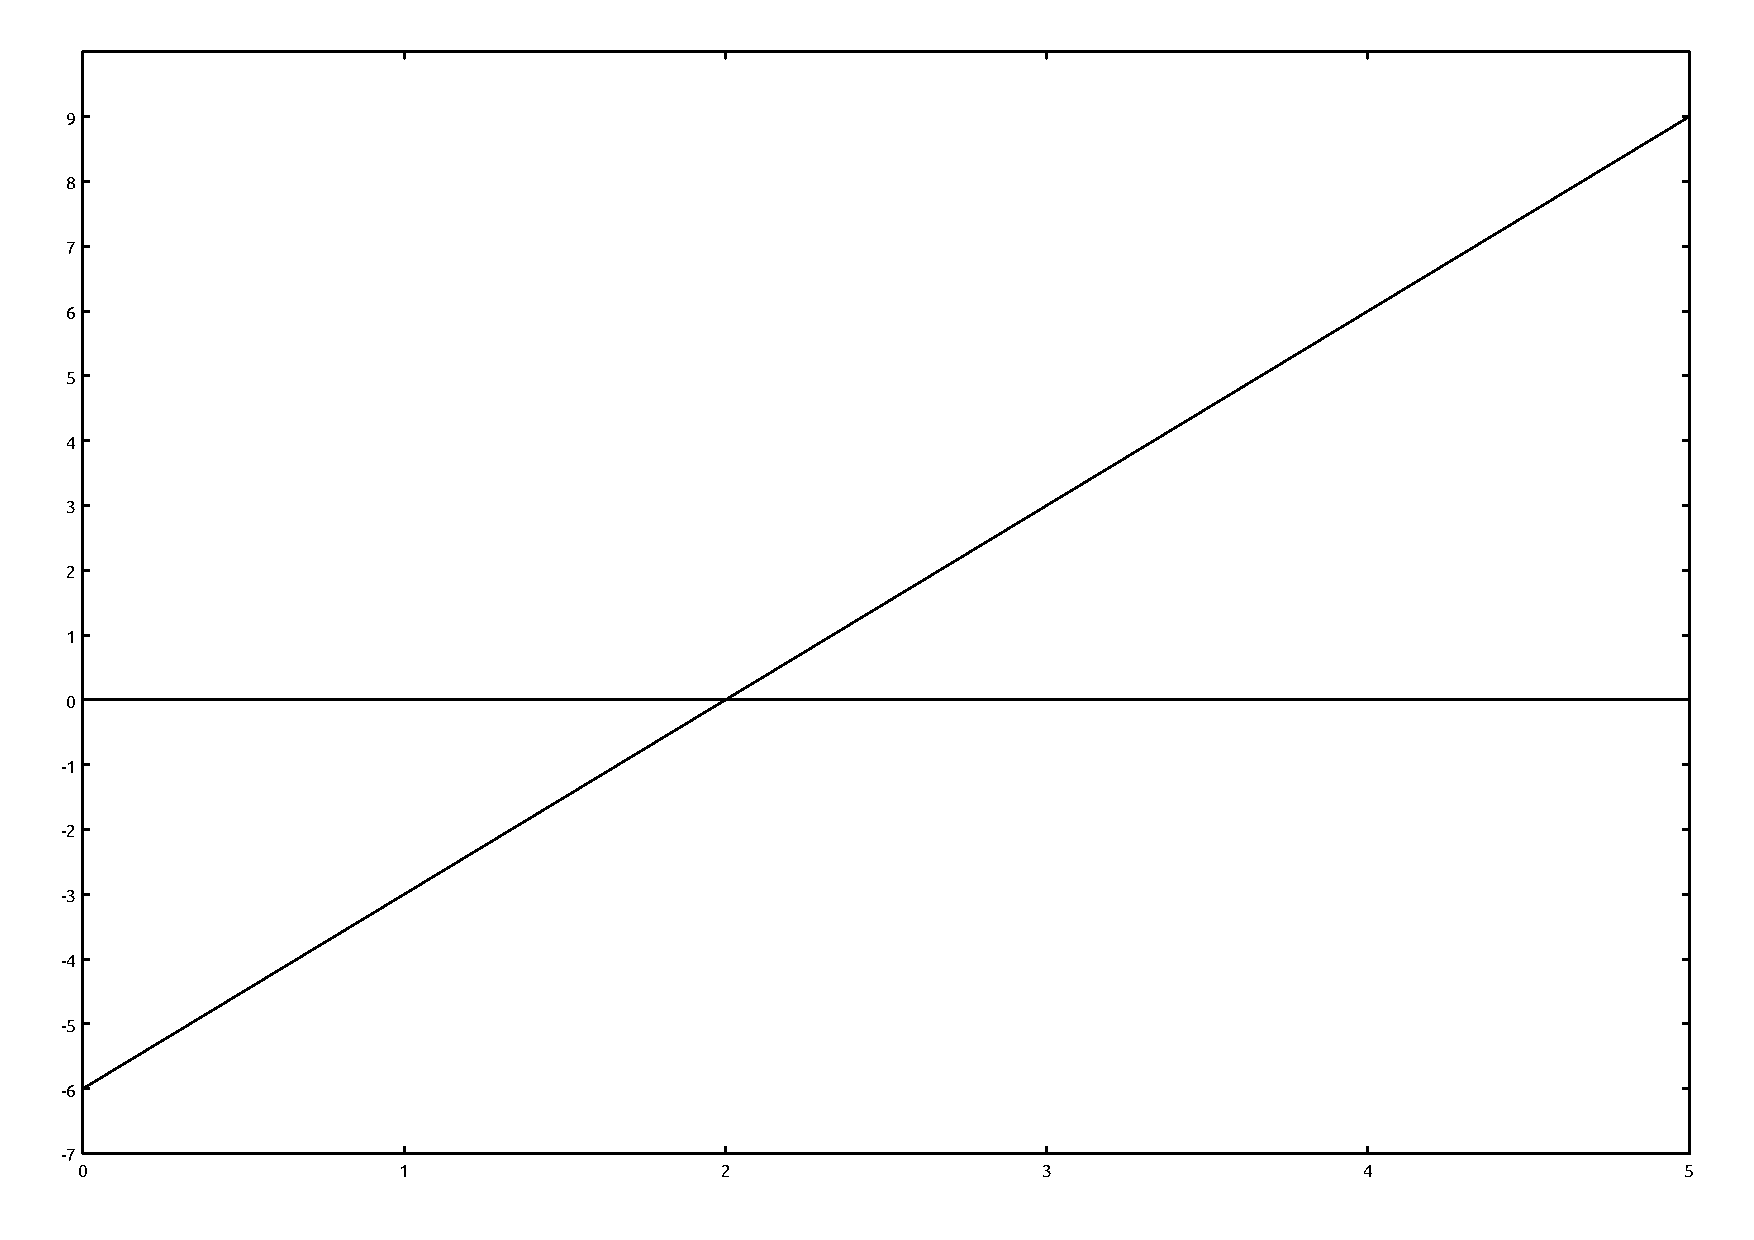
\includegraphics[width=0.7\linewidth]{sources/cours/droite.pdf}
  \end{figure}


  \subsection{Algorithme / Programme de Calcul}
  %-----------------------------------------------------------------------
  
\begin{verbatim}
   Choisir x;
   Soustraire 2;
   Multiplier le résultat par 3;
   Affichier le résultat; 
\end{verbatim}


\subsection{Expression littérale}
%-----------------------------------------------------------------------

$f(x) = (x - 2) \times 3 $

\end{multicols}


%-----------------------------------22222222222222222222222222222222222222
\section{Vocabulaires}
%-------------------------------------------------------------------------

On appelle $f$ la fonction qui a tout x associe la valeur $f(x)$.
\begin{multicols}{2}

  \subsection{Image}
  %-----------------------------------------------------------------------

  \begin{Definition}
    $y = f(x)$ est l'image de $x$ par la fonction $f$.
  \end{Definition}
  \begin{itemize}
  \item -3 est l'image de 1 par la fonction $f$.\\
  \item 6 est l'image de 4 par la fonction $f$.
  \end{itemize}
  \subsection{Antécédent}
  %-----------------------------------------------------------------------

  \begin{Definition}
    $x$ est l'antécédent de $y$ par la fonction $f$.
  \end{Definition}

  \begin{itemize}
  \item 2 est l'antécédent de 0 par la fonction $f$.\\
  \item 5 est l'antécédent de 9 par la fonction $f$.
  \end{itemize}

\end{multicols}

\paragraph{Remarques}~~\\

\begin{multicols}{2}

  \begin{figure}[H]
    \centering
    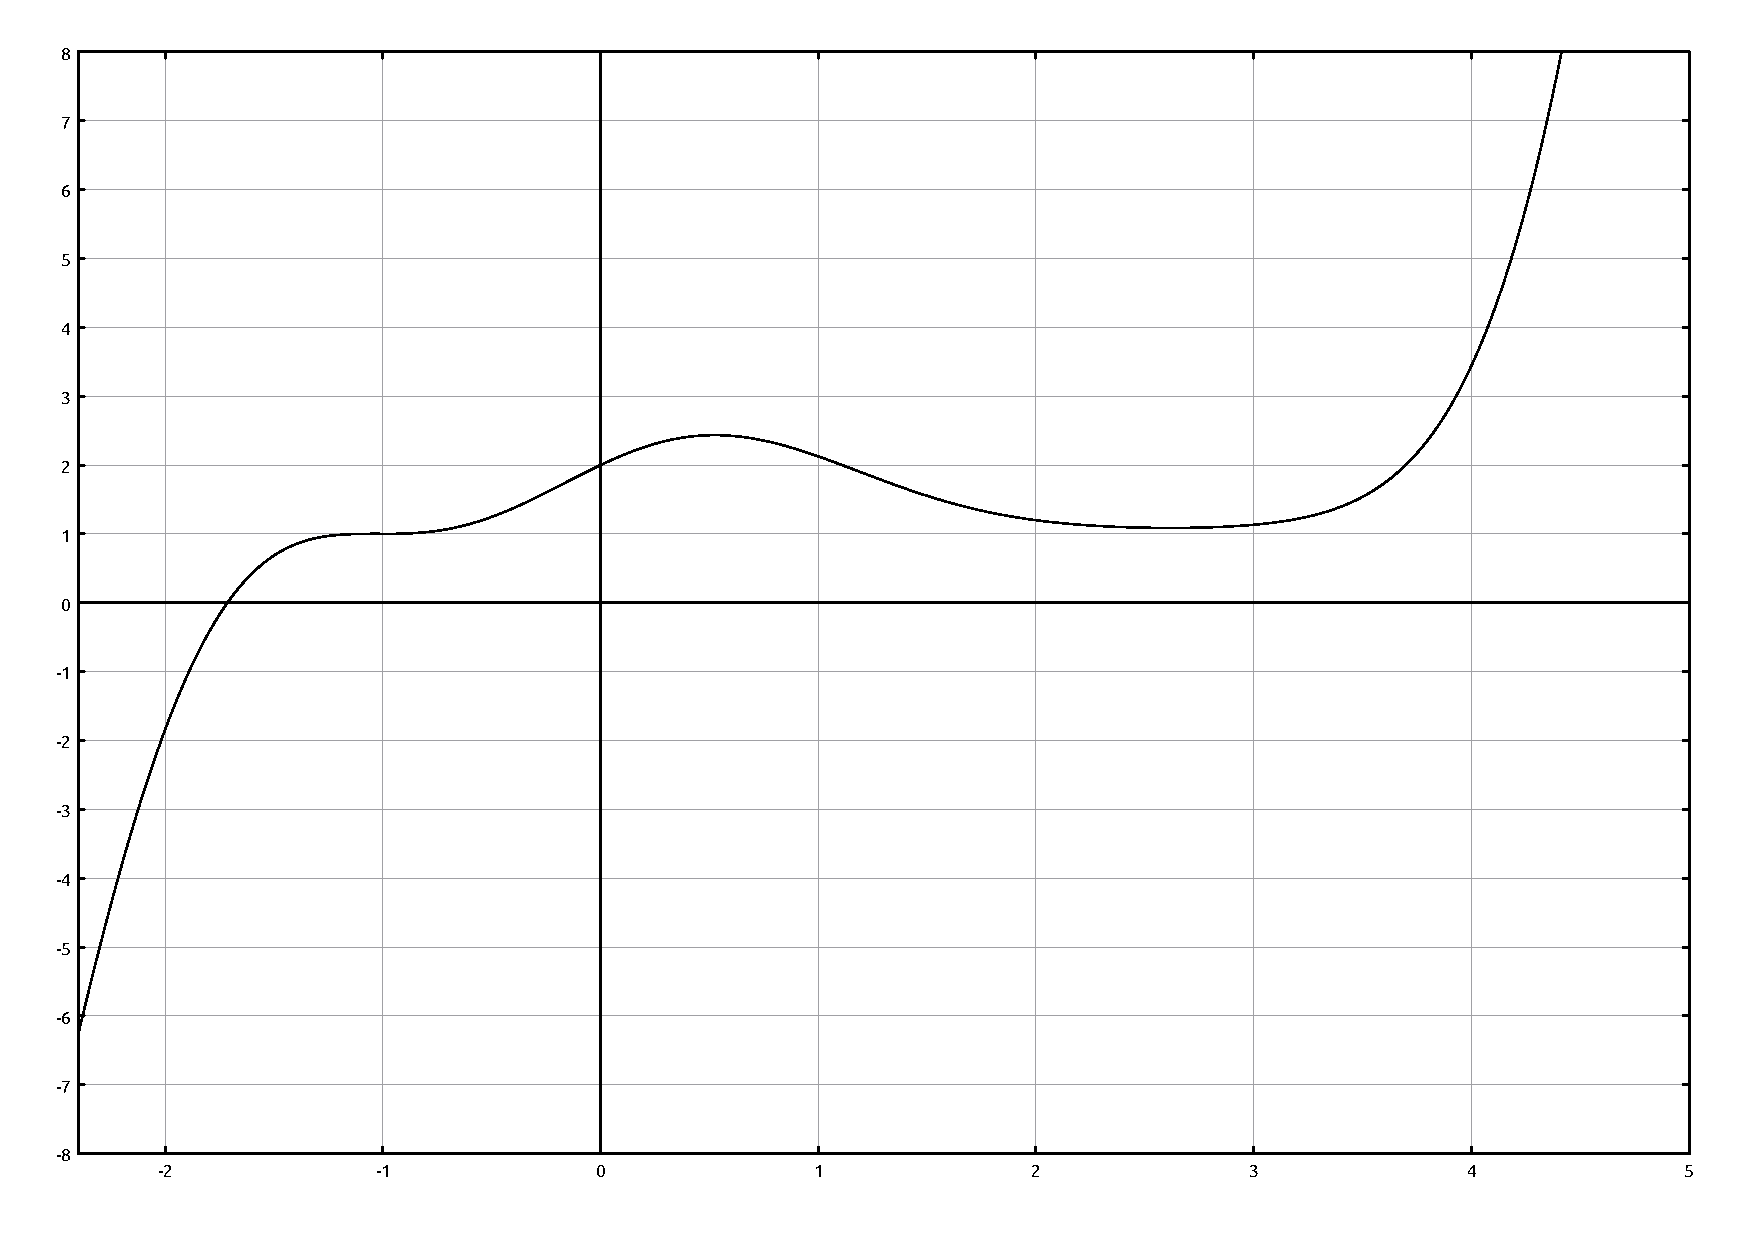
\includegraphics[width=0.7\linewidth]{sources/cours/courbe.pdf}
  \end{figure}


  \begin{itemize}
  \item Il peut avoir plusieurs antécédents.
  \item Il y a toujours qu'une seule et unique image.
  \item $0$, $1$ et $3.7$ sont les antécédents de $2$ par la fonction $f$.
  \end{itemize}
\end{multicols}

\newpage
%-----------------------------------33333333333333333333333333333333333333
\section{Domaine de définition}
%-------------------------------------------------------------------------

Parfois certaines fonctions ne sont définies que pour certaines valeurs de $x$. On utilise la notion d'intervalle.

\subsection{Intervalles}
%-----------------------------------------------------------------------
\begin{Definition}{$x \in \mathbb{R}$}\\
  x appartient à l'ensemble des réels, $x$ est réel.
\end{Definition}
\begin{multicols}{3}

  \begin{eqnarray*}
    x \in [-1      ; 5     ]\\
    x \in ] 0.5    ; 8     ]\\
    x \in ] 0      ; 9     [\\
    x \in [-5.2    ; -2    [\\
    x \in ]-\infty ; 7     ]\\
    x \in ] 2.5    ; \infty[\\
  \end{eqnarray*}

  \begin{eqnarray*}
    -1   \leq x \leq  5\\
    0.5  <    x \leq  8\\
    0    <    x <     9\\
    -5.2 \leq x \leq -2\\
    x    \leq 7\\
    x    > 2.5\\
  \end{eqnarray*}

  \begin{figure}[H]
    \centering
    \includegraphics[width=0.8\linewidth]{sources/cours/intervalles.pdf}
  \end{figure}
\end{multicols}


\subsection{Opérations sur les intervalles}
%-----------------------------------------------------------------------

\begin{multicols}{2}
  \subsubsection{Union}
  \begin{Definition}{Union}\\
    Appartenir à l'union de deux intervalles est possible si l'on appartient à l'un OU l'autre des intervalles.
  \end{Definition}
  $x \in [-5 ; 1 ] \cup ] 3 ; 4[$\\

  \subsubsection{Intersection}
  \begin{Definition}{Intersection}\\
    Appartenir à l'intersection de deux intervalles est possible si l'on appartient à l'un ET l'autre des intervalles, (au deux intervalles en même temps).
  \end{Definition}

  $x \in [-1 ; 6 ] \cap ] 3 ; 9[ = ]3 ; 6]$

\end{multicols}

\begin{multicols}{2}
  \begin{figure}[H]
    \centering
    \includegraphics[width=0.8\linewidth]{sources/cours/union.pdf}
  \end{figure}

  \begin{figure}[H]
    \centering
    \includegraphics[width=0.8\linewidth]{sources/cours/intersection.pdf}
  \end{figure}

\end{multicols}

\end{document}
